\documentclass[11pt, a4paper]{article}
\usepackage[a4paper, total={6.5 in,9in}]{geometry}
\usepackage[slovene]{babel}
\usepackage[utf8]{inputenc}
\usepackage[T1]{fontenc}
\usepackage{lmodern}
\usepackage{amsmath}
\usepackage{ amssymb }
\usepackage{amsfonts}
\usepackage{amsthm}
\usepackage{comment}
\usepackage{url}
\usepackage{gensymb}
\usepackage{subcaption}
\usepackage[pdftex]{graphicx}
\usepackage[section]{placeins}
\usepackage{mathtools}
\usepackage{float}
\usepackage{epstopdf}
\renewcommand{\vec}[1]{\mathbf{#1}}
\usepackage{hyperref}
\usepackage{wrapfig}

\pagestyle{plain}

\begin{document}

    \begin{center}
    {\LARGE\bfseries 9. Integracije s metodo Monte Carlo \par}
    \vspace{1cm}
    
    {\Large Domača naloga pri predmetu Modelska analiza I\par}
    \vspace{0.2cm}
    {\normalsize Avtor: Matic Noč \par}
    \vspace{0.2cm}    
    {\normalsize 15.11.2017 \par}    

    
    \end{center}
\section{Uvod}
Obravnavamo metodo integracije s Monte Carlo. Metode zavezemajo tako numerično integracije, kot simulacije različnih procesov, za katere poznamo fizikalne zakone le za majhne količine. 
\section{Metode Monte Carlo}
\subsection{Simulacije s metodo Monte Carlo}
Metoda Monte Carlo izvira iz ideje, kako izračunati zahtevne kombinatorične in verjetnostne probleme, npr. pri igrah s kartami. Ideja se je sprevrgla v algoritem, ki preprosto simulira naključni proces (npr. delitev kart), za katerega poznamo točno porazdelitev in verjetnost, in to ponovimo večkrat ter spremljamo kolikokrat smo dobili dogodek, katerega verjetnost želimo izračunati. Če tako simulacijo velikokrat ponovimo, se bomo približali pravi verjetnosti, katere analitičen izračun je lahko poljubno kompliciran.\newline\newline 
Za dobro natačnost moramo seveda generirati dobra naključna števila, po različnih porazdelitvah, kar smo se naučili v prejšni nalogi. Ponavadi obsegajo simualcije Monte Carlo več miljard naključnih žrebov, zaradi česar so se začele razivjati s računalniško tehnologijo.
\subsection{Integracije s metodo Monte Carlo}
Numerično integracijo lahko preprosto izvedemo s trapezno oziroma kakšno drugo površinsko metodo, katerih časovna zahtevnost narašča s številom dimenzij. Zgornje simulacije s metodo Monte Carlo nas napeljejo na idejo, da bi lahko števila v integralskih mejah žrebali naključno in računali povprečje naše funkcije  v danem območju, ki jo na koncu pomnožimo s celim območjem, ter tako dobimo vrednost integrala. Ker za konvolucijo naključnih števil velja centralni limitni izrek, se bo naša napaka med integralom in ocenjeno vrednostjo manjšala s $\sqrt{N}$ in bo tako neodvisna od dimenzij, kot pri ostalih shemah.
\begin{equation}
 \int_{\Omega} f(\mathbf{x})  d \mathbf{x}
\end{equation} 
Torej smo naš željen integral razdelili na $f(x)$, katerega vrednosti računamo. Torej moramo izžrebati točke, znotraj območja. 
\begin{equation}
{\mathbf{x}}_1, \cdots, \mathbf{x}_N\in \Omega
\end{equation}
so naključne točke v našem območju. Če je območje kvadrat ali krog, lahko točke izžrebamo že kar v njem, drugače pa našo domeno obdamo s kvadratom, iz katerega  žrebamo uniformno porazdeljene točke in gledamo kdaj padejo točke notri v domeno, ter upoštevamo le te. Potem lahko integral ocenimo kot povprečno vrednost funkcije pomnoženo s velikostjo domene.
\begin{equation}
I \approx Q_N \equiv V \frac{1}{N} \sum_{i=1}^N f(\mathbf{x}_i) = V \langle f\rangle
\end{equation}
\begin{equation}
\lim_{N \to \infty} Q_N = I
\end{equation}
\begin{equation}
\mathrm{Var}(f)\equiv\sigma_N^2 = \frac{1}{N-1} \sum_{i=1}^N \left (f(\mathbf{x}_i) - \langle f \rangle \right )^2 =  \langle f^2 \rangle  - \langle f \rangle^2
\end{equation}
Torej lahko varianco funkcije računamo sproti tako da izračunamo razliko $\sqrt{ \langle f^2 \rangle  - \langle f \rangle^2}$. Ker je povprečje porazdeljeno po normalni porazdelitvi, zaradi centralnega limitnega teorema, se varianca ocene integrala zapiše kot
\begin{equation}
\mathrm{Var}(Q_N) = Var (\frac{V}{N} \sum_{i=1}^N f(\mathbf{x}_i))= \frac{V^2}{N^2} \sum_{i=1}^N \mathrm{Var}(f) = V^2\frac{\mathrm{Var}(f)}{N} = V^2\frac{\sigma_N^2}{N}
\end{equation}
Torej vidimo, da varianca naše ocene integrala pada s $N$ oziroma
napaka pada s $\sqrt{N}$.
\begin{equation}
\sigma = V \frac{\sigma_N}{\sqrt{N}}
\end{equation}
\subsection{Zmanjšanje variance - usmerjeno izžrebanje}
Torej bomo, če bomo dovolj dolgo počakali našo napako zaradi žreba funkcije (v zgornjem razdelku označeno kot $\sqrt{\mathrm{Var}(f)}= \sqrt{ \langle f^2 \rangle  - \langle f \rangle^2}$ vedno zmanjšali in se tako približali pravi vrednosti integrala. Če naša funkcija močno skače in pada, potem enakomerni žreb ni več dobra ideja, ker bomo le redko vzeli dele, kjer funkcija dejansko prispeva k velikosti povprečne vrednosti funkcije, velikokrat pa bomo vzeli eksponentne repe, kjer funkcija ne prispeva k povprečju. Takrat lahko integralu vsilimo neko porazdelitev $g(x)$, tako da ga pomnožimo s porazdelitvijo in delimo s njo. Želimo da se takšna porazdelitev obnaša podobno kot funckija $f(x)$ in nam v tistih ozkih delih, kjer funckija hitro narašča in pada \textbf{zviša} verjetnost za žreb ter tako prispeva k manjšem odstopanju naključnega žreba od povprečja.
\begin{equation}
 \int_{\Omega} \frac{f(\mathbf{x})}{g(x)}  g(x)  d \mathbf{x}
\end{equation} 
Sedaj, kot v zgornjem primeru izžrebamo $x$ po porazdelitvi $g(x)$.
\begin{equation}
g(x): {\mathbf{x}}_1, \cdots, \mathbf{x}_N\in \Omega
\end{equation}
in nato izračunamo oceno integrala, kot:
\begin{equation}
Q_{N} = {\frac  {1}{N}}\sum _{{i=1}}^{N}{\frac  {f({\mathbf  {x}}_{i})}{p({\mathbf  {x}}_{i})}}
\end{equation}
Tu ni treba množiti s volumnom domene, ker je $g(x)$ normirana in je "Volumen"
\begin{equation}
\int_{\Omega} g(x)  d \mathbf{x} = 1
\end{equation}
Očitno je, da bomo v tem primeru zmanjšali varianco, torej razporeditev točk okoli povprečja, saj bomo jemali tiste točke, veliko prispevajo k povprečju, tiste, ki pa so $0$ in ne prispevajo 
\section{Izračun prostornin, mas, momentov}
Prostornino izračunamo kot
\begin{equation}
 \int_{\Omega}   d \mathbf{x}
\end{equation} 
Problem imamo, ker pri čudnih oblikah teles ne znamo določiti univerzalne porazdelitve, ki bi ustreza enakomerni porazdelitvi po telesu. Zato telo obdamo s kocko / kroglo in najprej simuliramo verjetnost, da je točka v telesu
\begin{equation}
P = \frac{m}{N}
\end{equation}
kjer je $m$ število znotraj telesa, in $N$ število vseh.
Nato izračunamo volumen kot
\begin{equation}
V =  V_{kocka} P_{domena} = V_{kocka} \frac{m}{N}
\end{equation}
Na tak način lahko torej simuliramo enakomerno porazdelitev v kakršni koli domeni, nato pa lahko izračunamo različne fizikalne količine npr. masa, vztrajnostni momenti,..
\begin{equation}
m = \int_{\Omega}  \rho(\mathbf{x}) d \mathbf{x}
\end{equation}
torej je naša ocena za maso enaka
\begin{equation}
m = V  \langle \rho \rangle = V \frac{1}{m} \sum _{{i=1}}^{m} \rho(\mathbf{x_i})
\end{equation}
kjer uporabimo iste naključne števila, ki smo jih uporabili za računanje volumna.
 torej 
\begin{equation}
m = V  \langle \rho \rangle = V \frac{1}{m} \sum _{{i=1}}^{m} \rho(\mathbf{x_i}) =   \frac{m}{N} \frac{1}{m} \sum _{{i=1}}^{m} \rho(\mathbf{x_i}) =  \frac{1}{N} \sum _{{i=1}}^{m} \rho(\mathbf{x_i})
\end{equation}
torej seštevamo prostornine znotraj domene, delimo pa jih z številom vseh točk.

\subsection{Prostornina preseka treh valjev}
Za testiranje metode vzamemo prostornino preseka teh valjev, katerega analitično poznamo $V = 8R^3 (2-\sqrt{2})$, kjer je $R$ radij vseh treh valjev.\newline\newline
Za slednjo prostornino sploh ne rabimo zapisati integrala, temveč obdamo $\frac{1}{8}$ lika s kvadratom $x \in [0,R], y \in [0,R], z \in [0,R]$ in nato gledamo ali točke zadostijo sistemu enačb 
\[
x^2 + y^2 \leq R^2,
\]
\begin{equation}
x^2 + z^2 \leq R^2,
\end{equation}
\[
y^2 + z^2 \leq R^2,
\]
če zadostijo, lahko točko uporabimo večkrat, za računanje povprečja vseh količin, ki nas zanimajo, torej gostote in vztrajnostnega momenta, poleg volumna.
\subsection{Rezultati}
Prepričajmo se, da napake metode res padajo s $N^{-1/2 }$. Ker imamo logaritemsko skalo se nam to prevede na 
\begin{equation}
V = V_{MC} \pm \sigma
\end{equation}
\begin{equation}
log( V -  V_{MC} ) = log (\sigma)
\end{equation}
\begin{equation}
log( V -  V_{MC} )  = log (\frac{\sigma_N}{\sqrt{N}}) = log (\sigma_N) - 1/2 log(N) 
\end{equation}
kjer je $\sigma_N$ koren variance volumnov. Najprej smo narisali graf $log (|V - V_{analitična}|)$ in na to na graf fitali premico ter pogledali ujemanje koeficientov.
\begin{figure}[H]
  
\centering
  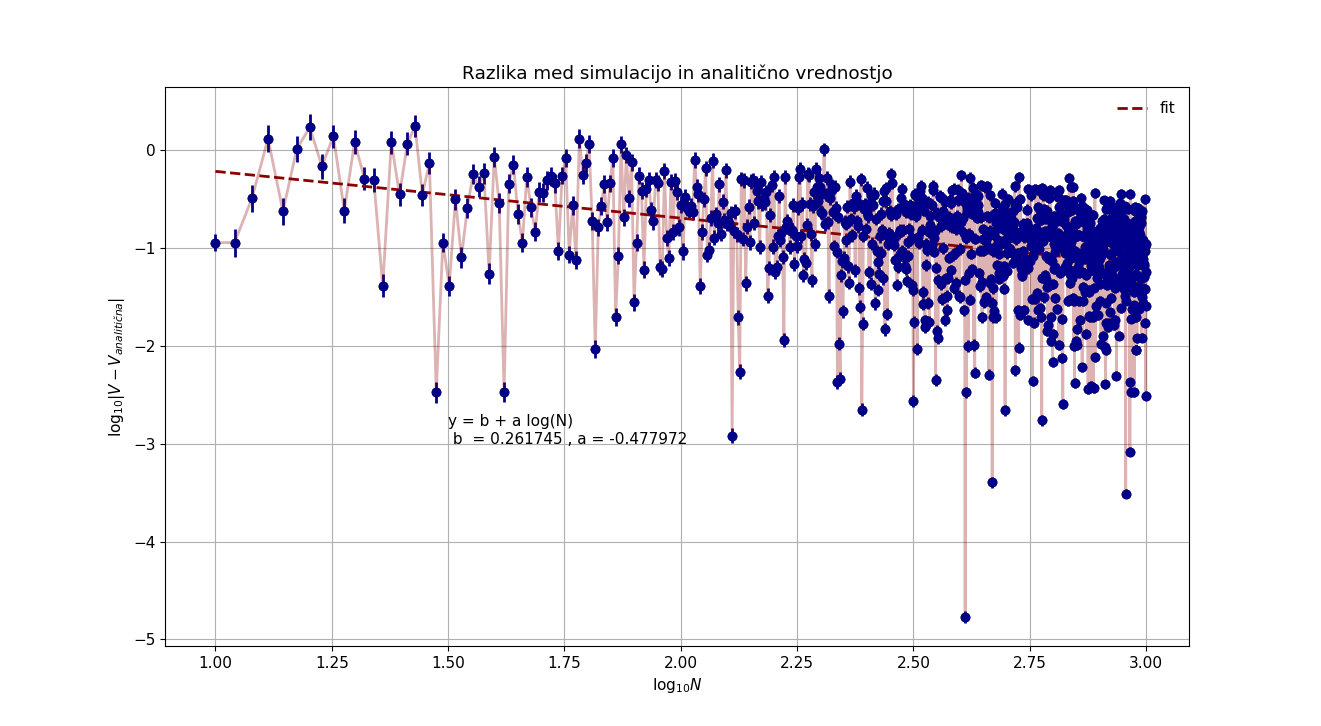
\includegraphics[width=15cm, height=10cm]{prva_razlike.png}
 \caption{Razlike med pravo in numerično rešitvijo padajo s $\frac{1}{\sqrt{N}}$, kar smo dokazali s fitom premice, katere koeifcient je $-0.5$, kar nam da $log N^{-1/2}$}
\end{figure}  
Poglejmo si še tabelo rešitev, ki jo dobimo pri dveh različnih gostotah
\begin{table}[H]
\caption{$n=10^7$, $\rho(r)=1$ in $R=1$. Vrednosti prostornine, mase in vztrajnostnega momenta preseka valjev za konstantno gostoto}
\label{my-label}
\begin{tabular}{llll}
\centering
 $\rho$ =1 & $V$ & $m$ & $J$\\\hline
 \textit{Monte Carlo} & 4.6881 $\pm$ $0.0011$ & 4.6881 $\pm$ $0.003$ & 0.6525 $\pm$ $0.0004$\\\hline
 \textit{Analitična rešitev} & 4.6863 & 4.6863 & /
\end{tabular}
\end{table}
V naslednji tabeli pa izračunamo gostoo
\begin{table}[H]
\caption{ $n=10^6$, $\rho(r) = r/R)^p $ in $R=1$. Izračun mase, prostornine in vztrajnostnega momenta J za različne potence $p$.}
\begin{tabular}{llll}
\centering
 $\rho(r) = (r/R)^p$ \vline & $V$ & $m$ & $J$\\ \hline
 \textit{p = 6} & 4.6833 $\pm$ $0.0011$ & 2.2020 $\pm$ $0.0007$& 0.4188 $\pm$ $0.0003$\\\hline
  \textit{p = 10} & 4.68182$\pm$ 0.00149  & 1.81741 $ \pm $ 0.00211 & 0.22578  $\pm$ 0.002003 \\\hline
 \textit{p = 19} & 4.6906 $\pm$ $0.0011$ & 2.3158 $\pm$ $0.0145$ & 0.5568 $\pm$ $0.0139$
\end{tabular}
\end{table}
Vidimo torej da nam radialna odvisnost gostote zmanjša maso in posledično vztrajnostni moment, vendar pa kljub pol manjši masi ($m_1 = 4.681 > m_2 = 2.2020$) ostaja vztrajnostni moment manj kot dvakrat manjši ($J_1 = 0.6525 , J_2 = 0.4188$), saj je gostota radialno odvisna in imamo veliko mase na robu lika. \newline\newline
Poglejmo kaj se dogaja z vztrajnostnim momentom $J$, če večamo potence p. 
\begin{figure}[H]
\centering 
  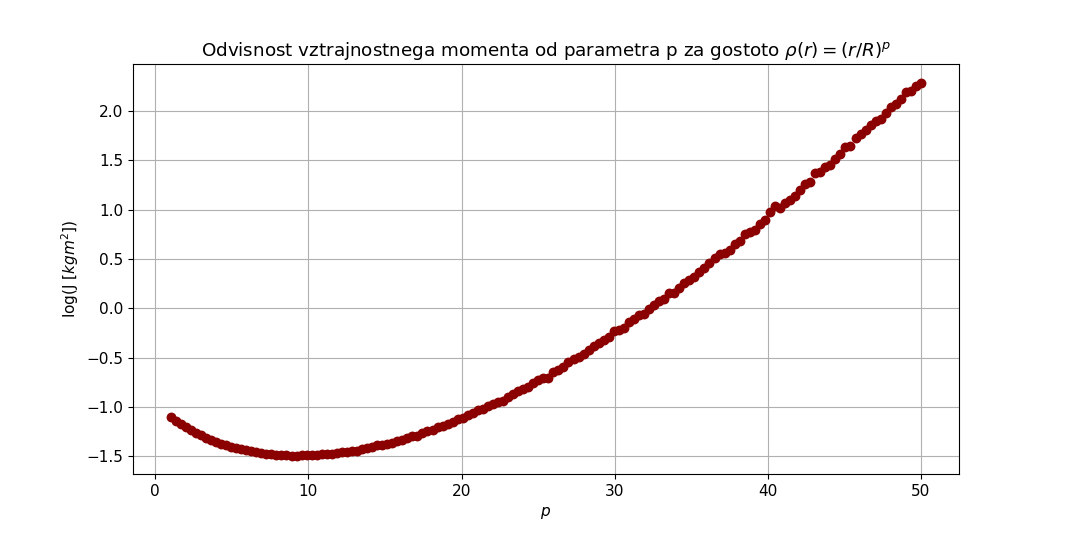
\includegraphics[width=10cm, height=7cm]{prva_vztrajnsotnimoment.png}
 \caption{Logaritemska skala kaže na začetno zmanjševanje vztrajnostnega momenta in nato močnan naraščaj (za $10^3$)}
\end{figure} 


\subsection{Absorbcija žarkov gama v krogli}
Recimo, da v krogli rodi žarek $\gamma$ npr. zaradi anihilacije pozitron elektron, izsevanja vzbujenih atomov ob jederskih razpadih... Za snov poznamo njen absorbcijski koeficient $\mu$ oziroma povprečno prosto pot $l = \frac{1}{\mu}$. Zanima nas kolikšen delež zapusti kroglo za različna razmerja radijev krogle in povprečne proste poti $\frac{l}{R}$.
\begin{figure}[H]
\hspace*{-2.5cm}  
  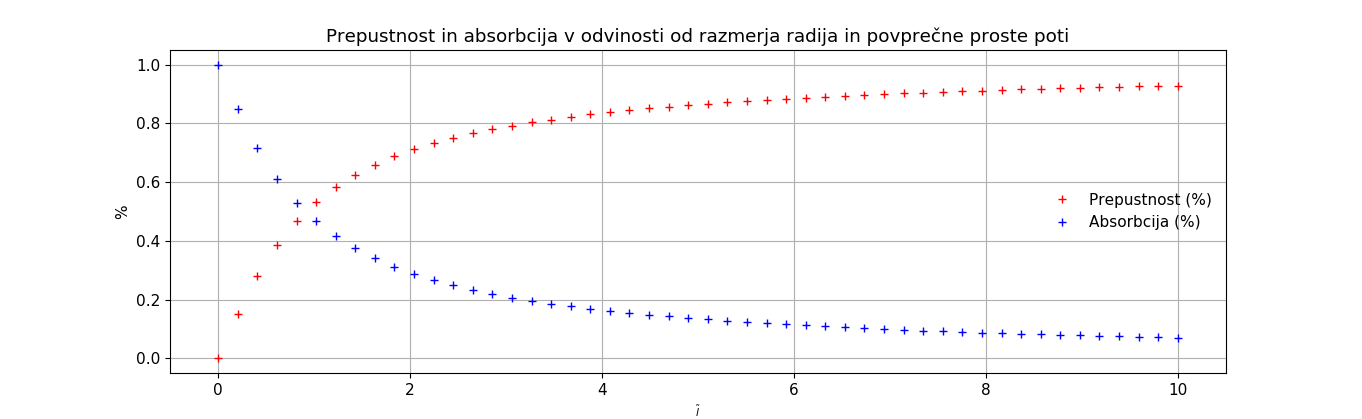
\includegraphics[width=22cm, height=6cm]{prepustnost_absorbcija.png}
 \caption{Simulacija prepustnosti in absorbcije za kroglo s različnimi razmerji povprečne proste poti in radijev za $n=10000000$ točk.}
\end{figure} 
Za povprečno prosto pot $\frac{l}{R}$ sklepamo, da je malo več kot pol, ker imajo vsi fotoni, ki nastanejo povprečno prosto pot 1
\begin{equation}
P ( \frac{l}{R} = 1) = 0.5270669
\end{equation}

\textbf{Poglejmo si sedaj nek primer iz jederskega razpada}. Imamo kepo kobalta, ki razpada s razpadom beta $t_{1/2} = 5.272 let$, torej bi morali kar nekaj časa čakati (ne realno) na meritve
\begin{equation}
{\displaystyle {}^{60}{\hbox{Co}}\;\to \;^{60}{\hbox{Ni*}}\;+\;e^{-}\;+\;{\overline {\nu }}_{e}.}
\end{equation}
Ni* pa se vrne v osnovno stanje z izsevanjem fotona $\gamma$ pri energiji $E_{\gamma} = 1.1732 MeV$
\begin{equation}
{\displaystyle {}^{60}{\hbox{Ni*}}\;\to \;^{60}{\hbox{Ni}}\;+\;\gamma .}  
\end{equation}
Kepo aproksimiramo s kroglo radija $R = 10cm = 0.1m$. Sedaj moramo oceniti absorbcijski koeficient za $\gamma$ pri dani energiji. Iz tabel lahko preberemo koeficiente.
\begin{table} [H]

\label{my-label}
\resizebox{\textwidth}{!}
{\begin{tabular}{llllll}
\centering

 E(keV)      & Total  attenuation [$\frac{cm^2}{g}$]  & Photoelect absorption [$\frac{cm^2}{g}$]  & Compton    scattering [$\frac{cm^2}{g}$]&    Coherent  scattering [$\frac{cm^2}{g}$] & Production Pair [$\frac{cm^2}{g}$]\\
1.0220E+03 & 5.8411E-02 & 3.7737E-04 & 5.7592E-02 & 4.4124E-04 & 0.0000E+00 \\
  1.2500E+03 & 5.2697E-02 & 2.5516E-04  & 5.2074E-02 & 2.9532E-04  & 0.0000E+00 

\end{tabular}}
\end{table}
Recimo, da se v približku comptonovim fotonom tako zmanjša energija, da se absorbirajo s fotoefektom. V tem primeru je povprečna prosta pot fotonov v kobaltu $\frac{1}{\mu} =\frac{1}{0.49 cm^{-1}} = 2cm$
Torej v bistvu spremljamo koliko primarnih fotonov , ki niso bili podvrženi sipanju ali absorbciji pride ven iz krogle. Rezultat nam da \begin{equation}
P (\frac{l}{R} = 0.2 ) = 0.130929 %
\end{equation}
Čeprav je povprečna prosta pot majhna v primerjavi s radijem, pa foton lahko nastane blizu mejnega radija in tako zleti ven.\newline\newline
Sedaj tudi vidimo, kaj bi storili v primeru več plastne razporeditve; za vsako plast posebej bi izračunali poti fotonov v plasti in gledali ali pride foton ven ali ne, če pride ven je podvržen naslednji sipalni plasti,
\subsection{Varianca prepustnosti}
Ker nimamo eksaktnega integrala, nam ne preostane drugega, kot da večkrat (npr. 100) ponovimo simulacijo pri različnih številih naključnih izborov $N$ in izračunamo povprečje, varianci in standardni odklon prepustnosti, ki služi kot ocena za napako. Ta bi se moral manjšati s $\sqrt{N}$
\begin{figure}[H]
\hspace*{-2.5cm}  
  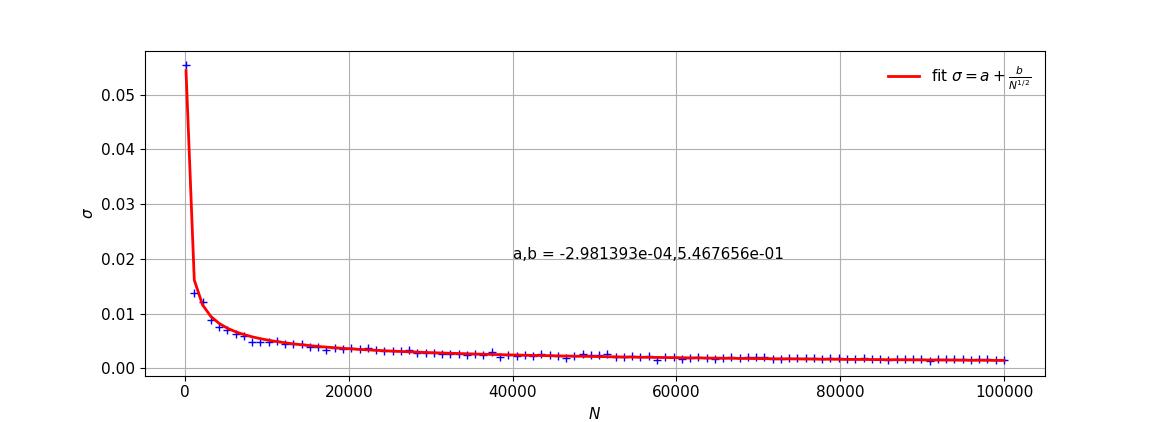
\includegraphics[width=22cm, height = 6cm]{varianca_druga.png}
 \caption{Vidimo, da se standardni odklon res manjša s korenom $N$ in v našem primeru, zaradi majhne variance same funkcije $\sigma_N$, hitro pada proti 0, zato ne potrebujemo zelo veliko naključnih žrebov (20 000 je dovolj za natačnost $\sim 1\%$)}
\end{figure}
\section{Naključno 1D sipanje v nevtronskem reflektorju}
\subsection{1D sipanje}
Vzemimo plast nevtronskega reflektorja, v katerega usmerimo nevtrone. Predpostavimo sipanje le v eni dimenziji, torej v smeri naprej - nazaj; v tem primeru simuliramo naključni sprehod v eni dimenziji. Nevtronski reflektor ima debelino $d$. V njem poznamo absorbcijski koeficient za sipanje $\mu$ oziroma povprečno prosto pot $l = \frac{1}{\mu}$. Vemo, da vsako novo mesto sipanja $s$ določa eksponentna porazdelitev po dolžinah, ki jo nevtron prepotuje preden se siplje
\begin{equation}
\frac{dP}{ds} = l e^{-s/l}
\end{equation}
Za to lahko izračunamo kumulativno porazdelitev in jo nato obrnemo, da dobimo transformacijo iz $\eta \in U(0,1)$ v $s \in  \frac{dP}{ds}$
\begin{equation}
s_i = - l * ln(1 - \eta_i)
\end{equation}
Sedaj pa vzemimo dva primera in sicer sprememba smeri pri vsakem sipanju in naključna sprememba smeri ob sipanju, ter spremljamo pozicijo nevtron  $x$, kjer vsakič premaknemo nevtron prepotovano pot do sipanja, torej
\begin{equation}
x_{i+1} = x_i \pm s_i ,
\end{equation} 
kjer je začetni položaj $ x_0 = 0$. Delec nato prištejemo v kategorijo prepuščeno $T$ ali $R$, odvisno od tega kam ga sprehod vodi. Velja še da je število vseh nevtronov $N$ enako $N = T + R$. Če slednje izraze delimo s celotnim številom ižrebanih nevtronov, tako simuliramo deleže prepuščenih in odbitih nevtronov. Zanima nas kakšno mora biti razmerje debeline in povprečne proste poti, da bo čim večji odboj $R$. \newline\newline
Vzemimo dve različni možnosti:\newline
A)Vsakič ko nevtron trči zamenja smer\newline
B)Ob trku se smer zamenja naključno 
\subsection{Rezultati}
Prikažemo $R $ in $T$ za različna razmerja povprečne proste poti in debeline reflektorja $q =\frac{l}{d}$. \newline\newline 
Za vsako razmerje $q$ smo simulirali $n = 10^5$ delcev in šteli število prepuščenih in odbitih delcev. Poglejmo si najprej simulacijo A), torej za \textbf{nujno menjavo smeri delca ob trku}:
\begin{figure}[H]
\hspace*{-2.5cm}  
  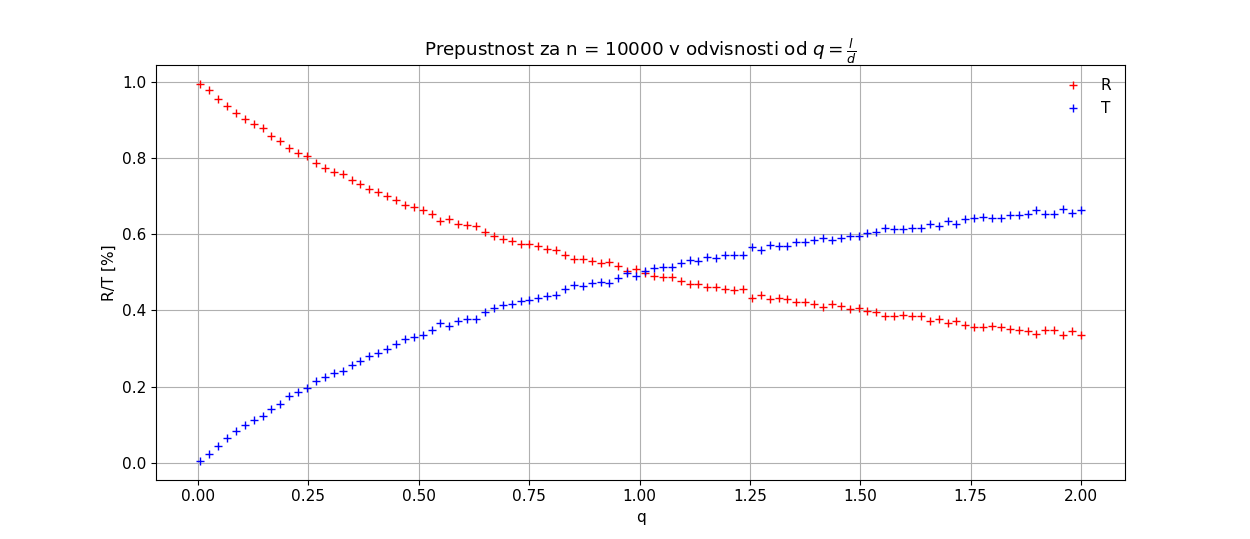
\includegraphics[width=22cm, height = 6cm]{tretja_2.png}
 \caption{Pri menjavanju smeri dobimo $50 \%$ odboj pri povprečni prosti poti $l = d $, kar ne predstavlja fizikalne rešitve, tudi če pomislimo ni razloga za determinističen odboj delca.}
\end{figure}
Model B) pa nam da fizikalno smiselno rešitev:
\begin{figure}[H]
\hspace*{-2.5cm}  
  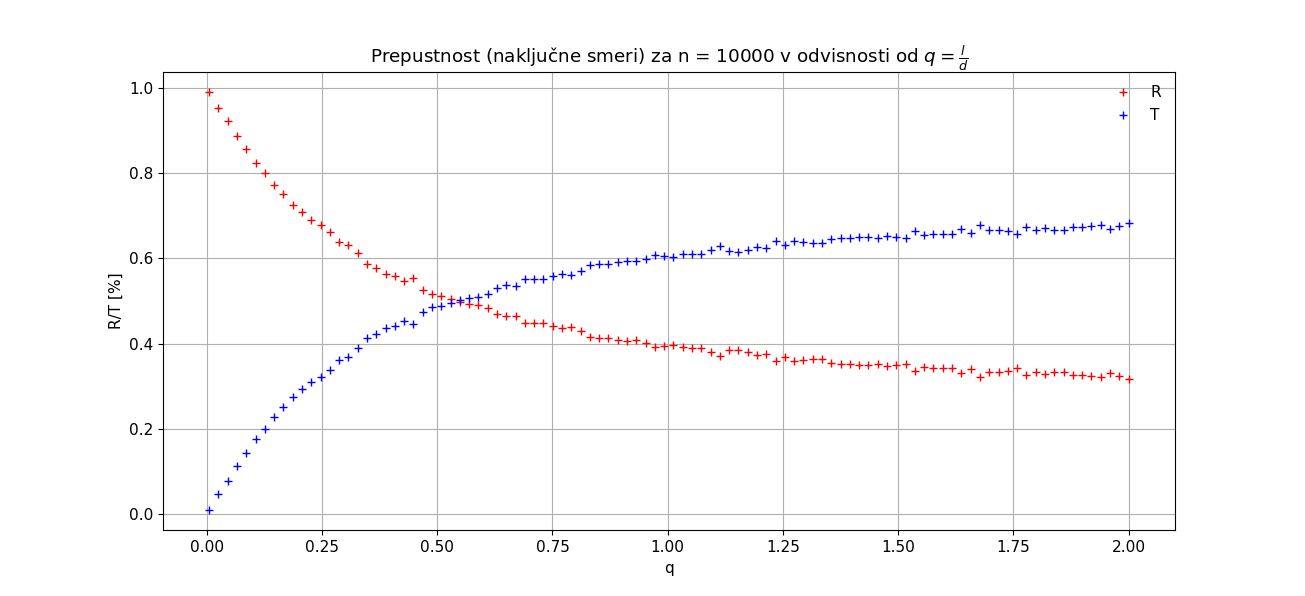
\includegraphics[width=22cm, height = 6cm]{tretja_1.png}
 \caption{Ko je povprečna prosta pot je odbojnost ravno enaka polovici, saj v povprečju delec prispe do polovice absorberja nato pa se s verjetnostjo $50 \%$ odbije levo ali desno in tako pobegne na ustrezno stran absorberja.\newline\newline
 Vidimo tudi, da kljub dolgi povprečni prosti poti napram debelini odbojnost ne pade na 0, saj je še vedno velik verjetnosta, da se bo nevtron sipal že na manjši razdalji.  }
\end{figure}
Ob danem absorbcijskem koeficientu $\mu$ oziroma povprečni prosti poti $l$, je potrebno izbrati tak $d$, da bo razmerje $\frac{l}{d}$ čim nižje. 
\newline\newline Presek za sipanje termalnih nevtronov (počasnih) za ogljik (grafit) znaša $5 Barn$, presek za absorbcijo pa je kar 1000x manjši, zato absorbcijo lahko zanemarimo. Vemo je $\mu  = \sigma n$, kjer je $n = \frac{N}{V}$ in je torej 
\begin{equation}
\mu = \sigma \frac{\rho Na}{M},
\end{equation}
gostota pa je približno $2 g /cm^3$ tako dobimo $\mu = 50.1/m^2$ oziroma povprečno prosto pot $l = 1.99 cm$ iz česar lahko sklepamo. Da bi nevtronski reflektor iz grafita moral biti debel več kot $4cm$, da bo odbil vsaj pol počasnih nevtronov, za $ 80 \% $ odbojnost pa 8cm.
\newline\newline
Oglejmo si še povprečno število in odstopanje sipanj za različna razmerja $q$. Ta naj bi se moralo močno zmanjšati, ko je povprečna prosta pot večja od debeline absorberja.
\begin{figure}[H]
\hspace*{-2.5cm}  
  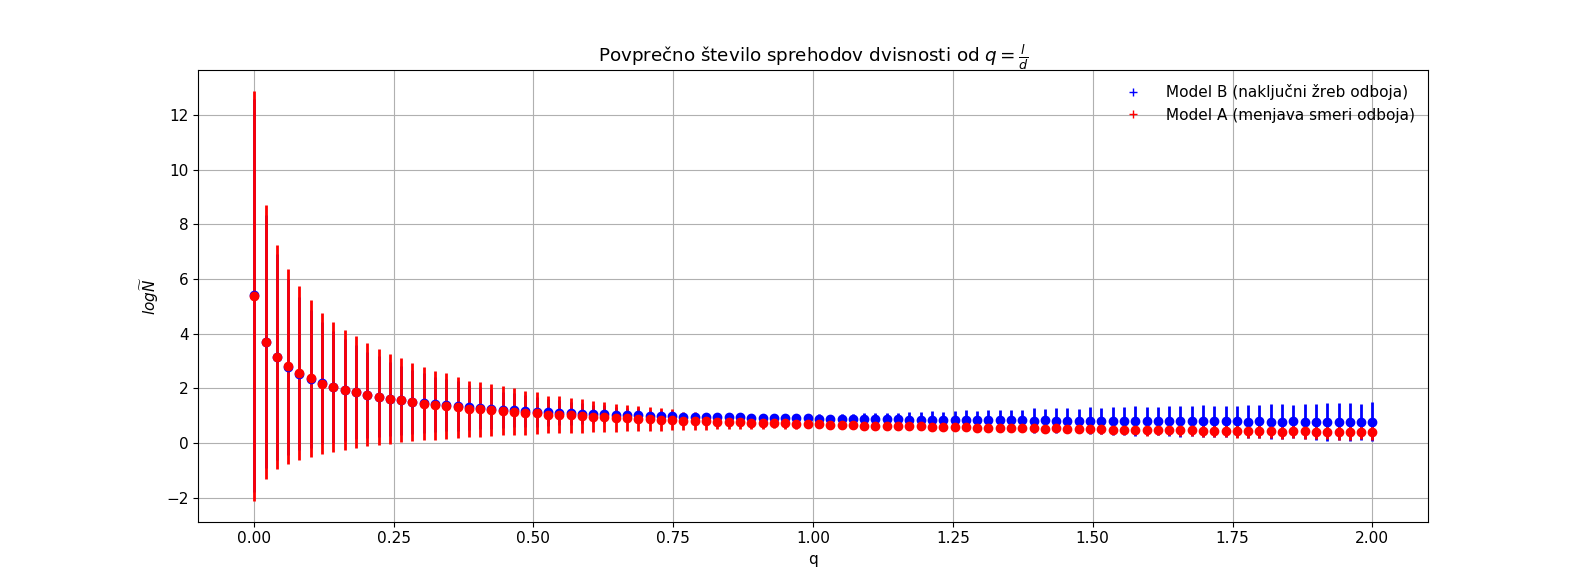
\includegraphics[width=22cm, height = 6cm]{tretja_stevilo.png}
 \caption{Povprečno število sipanj (logaritemska skala) je ob majhnih povprčenih prostih poteh veliko in ima tudi veliko varianco, med tem ko pri večjih $l$ hitreje pridemo ven iz absorberja. Vidimo tudi, da se na začetku število sipanj prekriva s obema modeloma, kasneje pa se bistveno odcepi, saj pri determinističnem odboju delec hitreje pobegne ven. }
\end{figure}
\subsection{Izotropno sipanje}
Vzemimo še model izotropnega sipanja, kjer je zaradi simetriji zadosti, da gledamo le smer $x$ in kot $\theta$, ki nam določa smer odboja. Smeri $y$ ne potrebujemo, saj nam izhod iz reflektorja določa le os $x$, zato vsakič projeciramo pot do novega trka na os $x$ in gledamo ali smo padli ven iz absorberja. 

\begin{equation}
x_{i+1} = x_i \pm s_i cos \theta_i,
\end{equation} 
\begin{figure}[H]
\hspace*{-2.5cm}  
  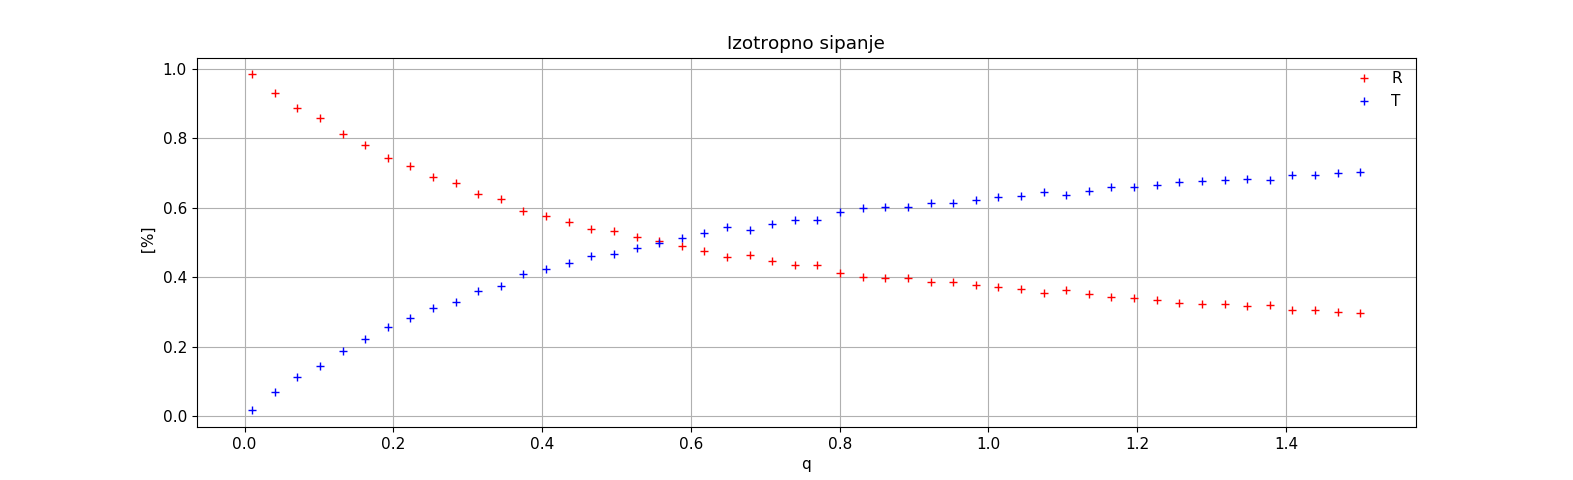
\includegraphics[width=22cm, height = 6cm]{tretja_izotropno.png}
 \caption{Izotropno sipanje je podobno modelu B), le da zaradi krajših smeri v smeri $x$, zaradi sipanja pod različnimi koti, odbojnost manj strmo pada s $\frac{q }{l}$. in je zato lahko debelina za ustrezno odbjonost $R$ manjša, kot v modelu B).}
\end{figure}
Pričakujemo višje število sipanj v odvisnosti od $q$ v tem modelu, zaradi krajših poti v smeri $x$.
\begin{figure}[H]
\hspace*{-3cm}  
  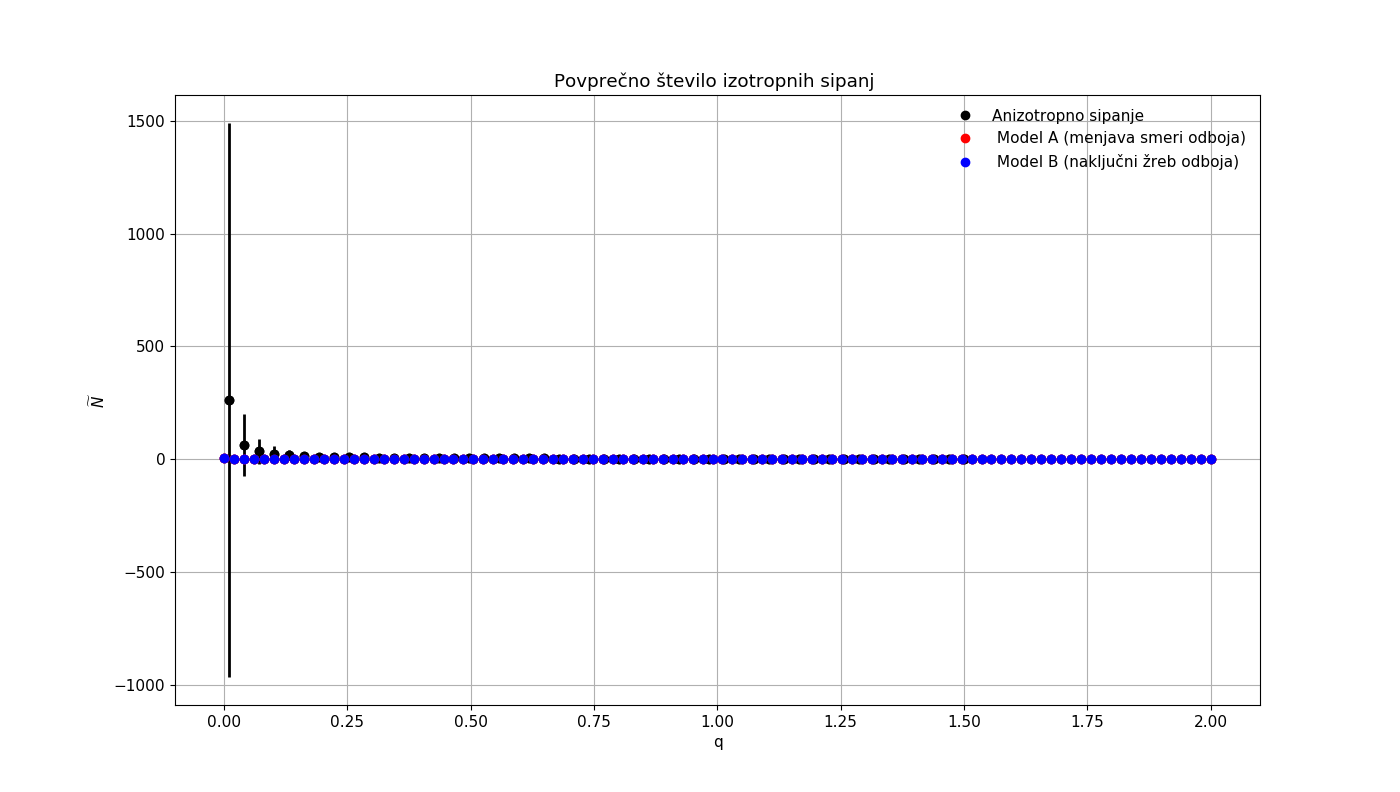
\includegraphics[width=22cm, height = 10cm]{tretja_izotropno2.png}
 \caption{Povprečno število sipanj za dani $q$ je pričakovano večje od modela A) in B).}
\end{figure}
\section{Zaključek}
Monte Carlo je močna metoda, ki ima prednost, da pogosto ne rabimo analitčno določevati kaj se dogaja. Ob poznavanju posameznih fizikalnih procesov, verjetnosti za določene procese, lahko simuliramo naključne sprehode, detekcije delcev in mnoge ostale analitično težko oziroma ne izračunljive stvari. Monte Carlo je prikladen tudi za reševanje n-ternih integralnov, zaradi tega ker je njegova napaka neodvisna od dimenzije, psevdo-generatorji naključnih števil pa so prot diskretizaciji prostora poceni. Pogledali smo si le fragment sposobnosti metode MC, saj lahko modele sedaj poljubno zakompliciramo (sipanje, absorbcija, detekcija le v določenih smereh).

\end{document}